\documentclass[a4paper,11pt]{article}
\usepackage[utf8]{inputenc}
\usepackage[italian]{babel}
\usepackage{amsmath}
\usepackage{amsfonts}
\usepackage{amssymb}
\usepackage{physics}
\usepackage{graphicx}
\usepackage{subfig}
\usepackage{hyperref}
\usepackage{parskip}
\usepackage{tabu, wrapfig}
\usepackage{multicol}
\usepackage[italiano, ruled]{algorithm2e}
\usepackage[left=1in, right=1in]{geometry}

\newcommand{\avg}[1]{\left\langle {#1} \right\rangle}
\newcommand{\code}[1]{\texttt{#1}}
\newcommand{\chindof}{\chi^2 / \text{ndof}}

%opening
\title{Campo scalare reale in 1+1D: Termodinamica e misura della massa}
\author{Rocco Francesco Basta}
\date{}

\begin{document}

\maketitle

\begin{abstract}
    Scopo di questo progetto è lo studio della termodinamica di un campo scalare reale in 1+1 dimensioni. Confronteremo due metodi per calcolare l'energia interna e la pressione del sistema: uno diretto, ottenuto facendo le opportune derivate della funzione di partizione, e uno indiretto, basato sull'integrazione numerica dell'anomalia di traccia. Infine, è stata studiata la funzione di correlazione della trasformata di Fourier del campo per misurare la massa.
\end{abstract}

\section{Introduzione al sistema}
    La lagrangiana euclidea del campo scalare reale è data da
    %
    \begin{equation}
        L_E = \frac{1}{2} (\partial_\mu \phi )^2 + \frac{1}{2}m^2 \phi^2 
    \end{equation}
    %
    Come in meccanica quantistica, possiamo scrivere la funzione di partizione in termini di path integral sugli autovalori dell'operatore campo
    %
    \begin{equation}
        Z = \int \mathcal{D}\phi \, e^{-S_E[\phi]}
        \label{eqn:z-path-integral}
    \end{equation}
    %
    con le condizioni al bordo $\phi(\tau = 0) = \phi(\tau = \beta)$, e
    
    Di conseguenza, la media termica di un'osservabile $O$ è data da
    %
    \begin{equation}
        \avg{O}_\beta = \frac{1}{Z} \int \mathcal{D} \phi \, O[\phi] e^{-S_E[\phi]}
    \end{equation}
    %
    Nella simulazione, si introduce una discretizzazione su un reticolo cubico $(N_s, N_\tau)$ con passo reticolare $a$ e un volume spaziale finito $V$\footnote{Nel caso 1+1D è la lunghezza della scatola in cui è contenuto il sistema.}, con condizioni periodiche al bordo. Definendo il parametro $\hat{m} \equiv ma$, il limite del continuo si ottiene facendo il limite
    %
    \begin{subequations}
        \begin{equation}
            \hat{m} \equiv ma \to 0
        \end{equation}
        \begin{equation}
            V \equiv N_s a = \text{cost.}
        \end{equation}
        \begin{equation}
            \beta \equiv N_\tau a = \text{cost.}
        \end{equation}
    \end{subequations}
    %
    
    Definendo $\epsilon = E/V$ la densità di energia e $p$ la pressione del sistema, possiamo studiare le due quantità adimensionali $\epsilon / T^2$ e $p / T^2$. Studieremo inoltre l'anomalia di traccia $(\epsilon - p)/T^2$, che è diversa da zero quando l'invarianza di scala è rotta (in questo caso, è rotta esplicitamente dalla presenza della massa).
    
    Ci aspettiamo che, per $T/m \to \infty$, si abbia $\epsilon / T^2 \to \pi/6$ (legge di Stefan-Boltzmann), mentre $(\epsilon - p) / T^2 \to 0$ perché ad alte temperature la massa diventa sempre meno rilevante.
    
    Ricordiamo inoltre la relazione termodinamica, valida per sistemi omogenei in 1+1D,
    %
    \begin{equation}
        T\frac{\partial}{\partial T} \left(\frac{p}{T^2}\right) = \frac{\epsilon - p}{T^2}
        \label{eqn:pressure_from_anomaly}
    \end{equation}
    %
    che lega l'anomalia di traccia alla pressione, e permette quindi di ricavare in modo alternativo la densità di energia e la pressione del sistema.
    

    \section{Calcolo esplicito della pressione}
    
    Il modo più veloce per ottenere un'espressione del valor medio della pressione sul reticolo è utilizzare le espressioni note per la densità di energia e per l'anomalia di traccia:
    
    \begin{subequations}
        \begin{equation}
            \frac{\epsilon}{T^2} = \frac{1}{2}N_\tau^2 \avg{O_1 + O_2 - O_3} 
        \end{equation}
        \begin{equation}
            \frac{\epsilon - p}{T^2} = N_\tau^2 \avg{O_1}
        \end{equation}
        \begin{equation}
         \implies \frac{p}{T^2} = \frac{1}{2} N_\tau^2 \avg{-O_1 + O_2 - O_3}
         \label{eqn:pressure}
        \end{equation}
    \end{subequations}

    Dove $O_1 = \avg{\hat{m}^2 \phi^2}_{lat}$, $O_2 = \avg{(\phi(n + \hat{x}) - \phi_n)^2}_{lat}$, $O_3 = \avg{((\phi(n + \hat{\tau}) - \phi_n)^2}_{lat}$. L'espressione $\avg{\cdot}_{lat}$ indica la media dell'operatore sul reticolo, mentre $\avg{\cdot}$ senza pedice indica le medie termiche. Possiamo verificare esplicitamente questa espressione a partire dalla funzione di partizione.
    
    Il procedimento per ricavare un'espressione diretta della pressione è analogo a quello visto per l'energia interna.
    
    Per l'energia interna si introduce un parametro di anisotropia $a_t = \xi a$. Per comodità, noi considereremo il suo reciproco:
    %
    \begin{equation}
        a = \lambda a_t \implies \partial_x \to \frac{1}{\lambda a_t} \hat{\partial_x}
    \end{equation}
    %
    Utilizzando le equazioni
    %
    \begin{subequations}
        \begin{equation}
            p = - \left( \frac{\partial F}{\partial V} \right)_T
        \end{equation}
        \begin{equation}
            F = - \frac{1}{\beta} \log Z
        \end{equation}
        \begin{equation}
            V = N_s a = N_s \lambda a_\tau \implies \frac{\partial}{\partial V} = \frac{\lambda}{V} \frac{\partial}{\partial \lambda}
        \end{equation}

    \end{subequations}
    %
    e l'equazione (\ref{eqn:z-path-integral}), possiamo eseguire la derivata rispetto al volume, a temperatura costante, ottenendo così l'equazione (\ref{eqn:pressure}). A differenza del caso dell'energia interna, $\hat{m}$ e $\hat{\phi}(n)$ dipendono da $a$. Il calcolo va eseguito tenendo costanti $m$ e $\phi(n)$ (in 1+1D l'operatore campo è già adimensionale).
    
    Si ha
    %
    \begin{equation}
        \frac{\partial \log Z}{\partial \lambda} \bigg|_{T, m, \phi} = - \frac{1}{2} \avg{ a_t^2 \lambda \sum_n m^2 \phi(n)^2 - \sum_n \frac{1}{\lambda^2} (\phi (n + \hat{x}) - \phi(n))^2 + (\phi(n + \hat{\tau}) - \phi(n))^2}
    \end{equation}
    %
    da cui, posto $\lambda = 1$ per tornare ad un reticolo isotropo,
    %
    \begin{equation}
        \frac{p}{T^2} = \frac{\beta}{2 N_s a_\tau} N_s N_\tau \avg{O_1 - O_2 + O_3} \implies \frac{p}{T^2} = - \frac{N_\tau^2}{2} \avg{O_1 - O_2 + O_3}
    \end{equation}


    
    
    
    \section{Simulazioni numeriche}
    
    Sono state effettuate delle simulazioni con l'algoritmo Heatbath combinato con 4 spazzate di Overrelaxation con $N_s$ = 100, 150, 200, 250 e rispettivamente $\hat{m} = 0.1, 1/15, 0.05, 0.04$. Per ogni coppia ($N_s, \hat{m}$), sono state effettuate 14 simulazioni a diversi valori di $T/m$. Per eliminare divergenze, ad ogni osservabile è stato sottratto il valore per $N_s = N_\tau$.
    
    Successivamente, è stato effettuato il limite al continuo delle osservabili (densità di energia, pressione, anomalia di traccia) per ogni valore di $T/m$. 
    
    Infine, si è usato l'equazione (\ref{eqn:pressure_from_anomaly}) per ricavare pressione e densità di energia a partire dall'anomalia di traccia.
    
    Il risultato delle simulazioni è mostrato in figura (\ref{fig:thermo_observables}), mentre il limite al continuo e il confronto con le quantità ottenute dall'integrazione numerica dell'anomalia di traccia è mostrato in figura (\ref{fig:thermo_continuum}). Le linee tratteggiate rappresentano le quantità ottenute dall'integrazione numerica. Le barre d'errore rappresentano l'errore statistico ottenuto dalla propagazione dell'errore, mentre le bande colorate rappresentano una stima dell'errore sistematico.
    
    Più precisamente, l'integrazione numerica è stata fatta con il metodo dei trapezi. I limiti superiori e inferiori sono stati ottenuti sostituendo al fattore $y_i + y_{i+1} / 2$ il massimo o il minimo tra due punti consecutivi. Entrambi i metodi convergono, per $\Delta T/m \to 0$, al valore vero, e permettono di avere una stima grossolana dell'errore sistematico commesso nell'integrazione numerica.
    
    Con questa stima, le quantità ottenute dall'integrazione numerica sono compatibili con quelle ottenute direttamente derivando la funzione di partizione. La densità di energia sembra tendere come previsto a $\pi / 6$ a grandi temperature. 
    
    Un modo per analizzare il sistematico in modo più accurato potrebbe essere il seguente: dato che l'errore commesso sul singolo intervallo con il metodo dei trapezi è, al prim'ordine non nullo, $\propto \Delta^3$, si potrebbe fare altre simulazioni, con una ``griglia'' più fitta in $T/m$, ed estrapolare il limite al continuo eseguendo un fit con $f(\Delta) = f + k \Delta^3$.
    
    \begin{figure}[htb]
        \centering
        \subfloat[]{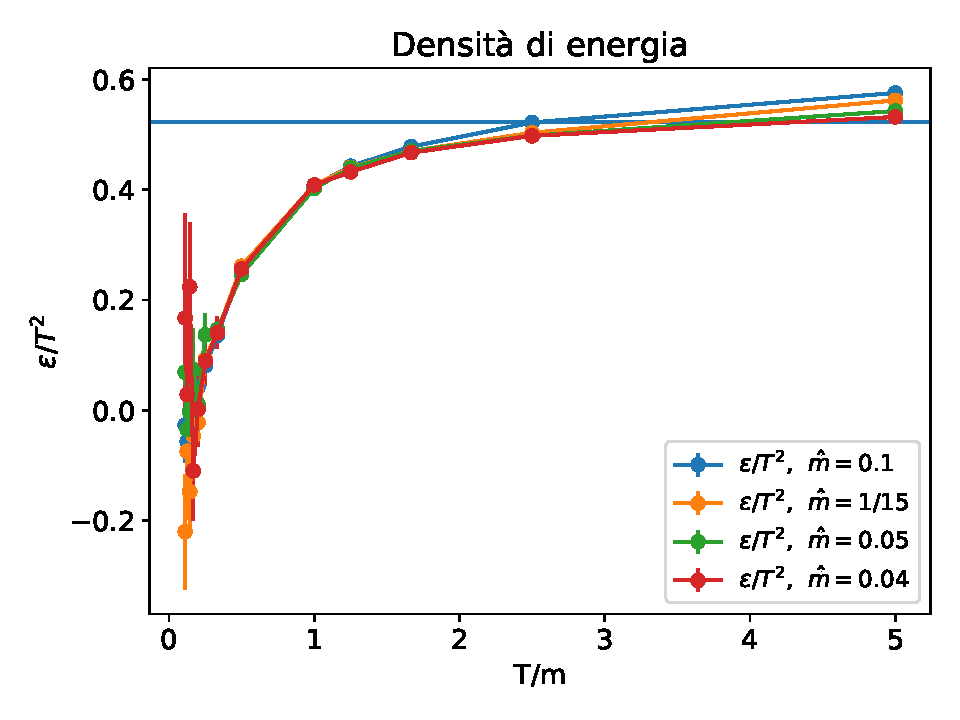
\includegraphics[width=0.5\textwidth]{figures/energy_raw.pdf}}
        \subfloat[]{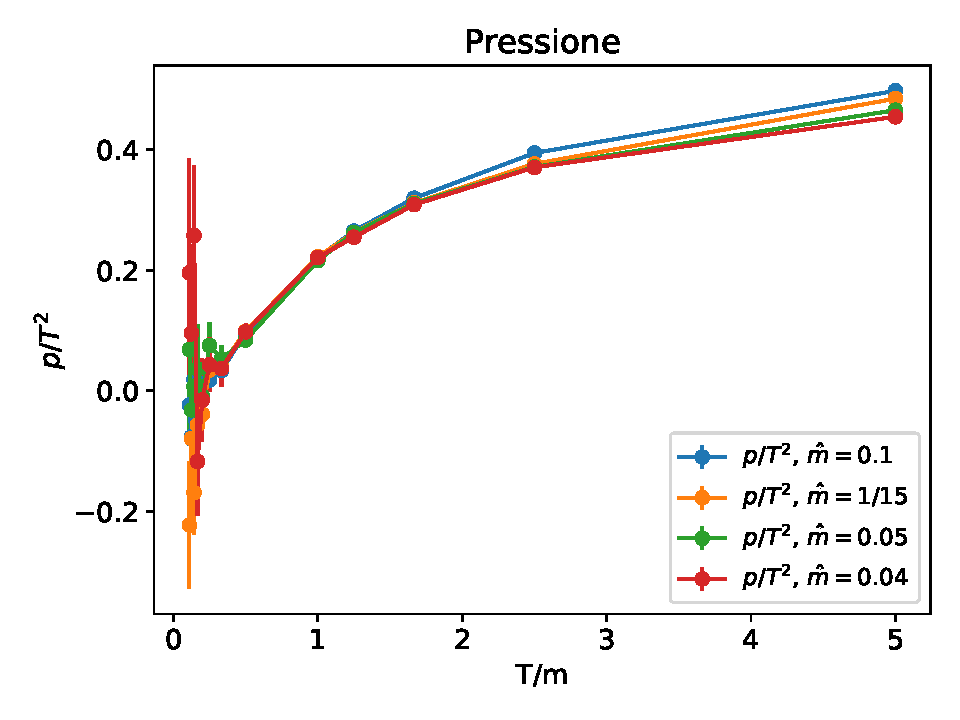
\includegraphics[width=0.5\textwidth]{figures/pressure_raw.pdf}} \\
        \subfloat[]{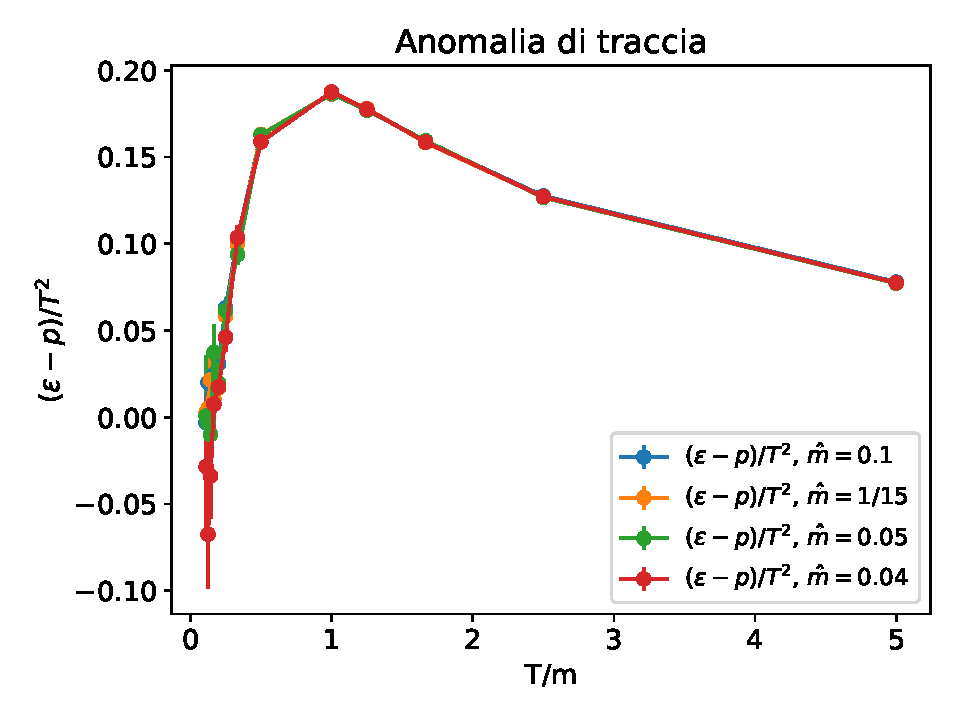
\includegraphics[width=0.5\textwidth]{figures/trace_anomaly_raw.pdf}}
        \subfloat[]{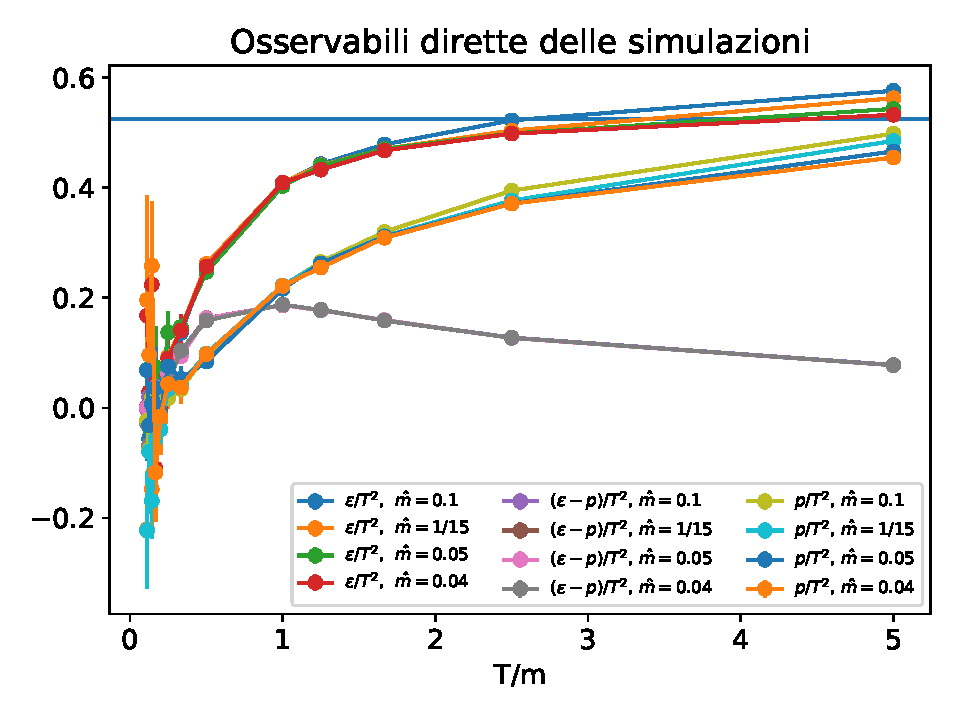
\includegraphics[width=0.5\textwidth]{figures/all.pdf}}
        \caption{Risultati delle simulazioni numeriche. La linea orizzontale indica il valore atteso per la densità di energia nel limite di massa nulla $\epsilon/T^2 \, [T/m \to \infty] = \pi / 6$.}
        \label{fig:thermo_observables}
    \end{figure}
   
    \begin{figure}[htb]
        \centering
        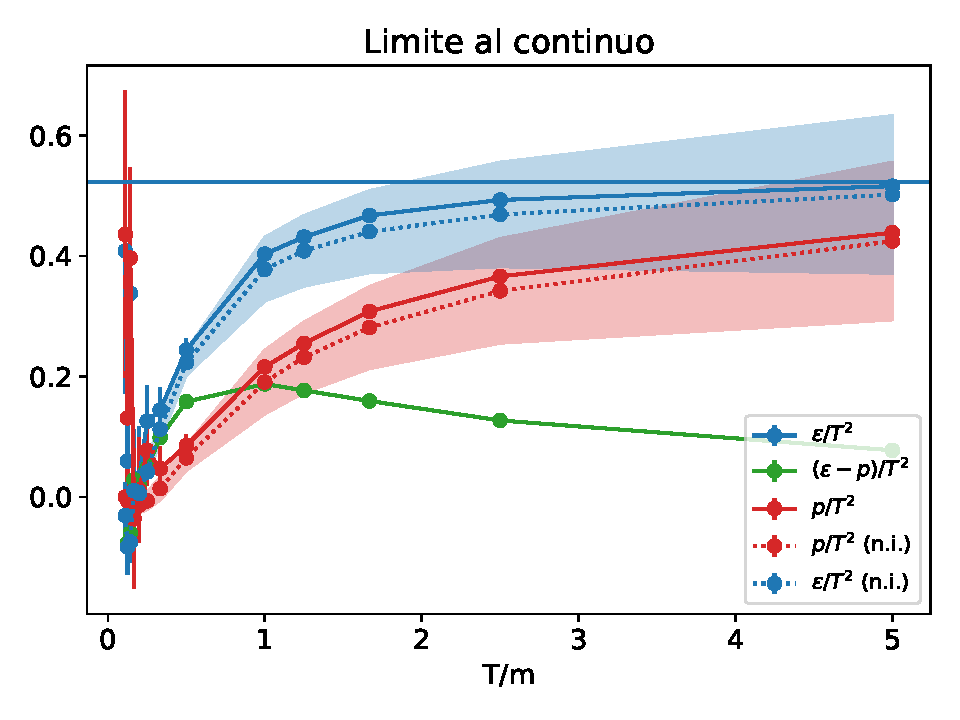
\includegraphics[width=0.8\textwidth]{figures/continuum.pdf}
        \caption{Limite al continuo delle quantità termodinamiche. Le linee tratteggiate rappresentano le quantità integrate numericamente. Le barre d'errore rappresentano l'errore statistico, ottenuto per propagazione dell'errore, mentre le bande colorate rappresentano un limite superiore al sistematico.}
        \label{fig:thermo_continuum}
    \end{figure}

    

    
    \section{Misura della massa}
   
    Le simulazioni sono state effettuate su reticoli quadrati ($N_s = N_\tau$) con i parametri fisici $V = 10$ e $\beta m = 10$, che implicano $m = 1$. 
    
    Il correlatore misurato è
    
    \begin{equation}
        C(\tau, p, q) = \avg{\int d^2 x \, e^{-ipx} \phi(x,\tau) \int d^2 y \, e^{iqy} \phi(y, 0)} / N
    \end{equation}
    
    Questo correlatore è atteso essere nullo per $p \neq q$, e a basse temperature ha un andamento proporzionale a $\exp (- E_p \tau)$, dove $E_p$ è l'energia della particella con impulso $p$.
    
    
    \begin{wraptable}{r}{4.5cm}
        \begin{tabular}{c c} \hline
        N & $m_N$ \\ \hline
        40 &    0.9890(42)  \\
        50 &    0.9908(52)   \\
        80 &    0.9912(88)  \\
        100 &   0.9958(75)  \\
        125 &   1.0002(84)  \\ \hline
        $N \to \infty$ & 0.9972(55)  \\ \hline
        \end{tabular}
    \caption{Fit del correlatore con $p = q = 0$ per la misura della massa.}
    \label{tab:mass_fit}
    \end{wraptable}
    

    Ponendo $p = q = 0$, si ha che $C(\tau, 0, 0) \propto \exp (-m\tau)$. Possiamo quindi sfruttarlo per misurare la massa del campo scalare.
    
    Le simulazioni sono state eseguite per $N_s = N_\tau \equiv N =$ 40, 50, 80, 100, 125, e rispettivamente $\hat{m} = $ 0.25, 0.20, 0.125, 0.1, 0.08, in modo da verificare le condizioni $\beta m = 10, V=10$.
    
    Per ogni simulazione, sono state prese 125000 misure, e sono state scartate le prime 50000 per termalizzazione. Gli errori sul correlatore sono stati stimati con l'usuale metodo di blocking.
    
    
    Dato che $\beta = 10$, la regione di fit è stata ristretta a $0 \leq \tau < 1$. Infatti, effetti di temperatura finita sono evidenti per $\tau \sim 5$ (figura (\ref{fig:mass_correlator_plot}), e per $\tau \gtrsim 1.2$ questi effetti non rendono possibile eseguire il fit con un singolo esponenziale.

    
    Le curve per diversi $N$, se normalizzate rispetto a $C(0, 0, 0)$, sembrano collassare. L'altezza del picco centrale sembra quindi indipendente dal reticolo. Il contributo di backpropagation ($\exp (-m (\beta - \tau))$) non è sufficiente per spiegare questo effetto, perché porterebbe a un andamento complessivo $\propto \cosh (m(\tau - \beta/2))$. 
   
    \begin{figure}[htb]
        \centering
        \subfloat[$C(\tau)$]{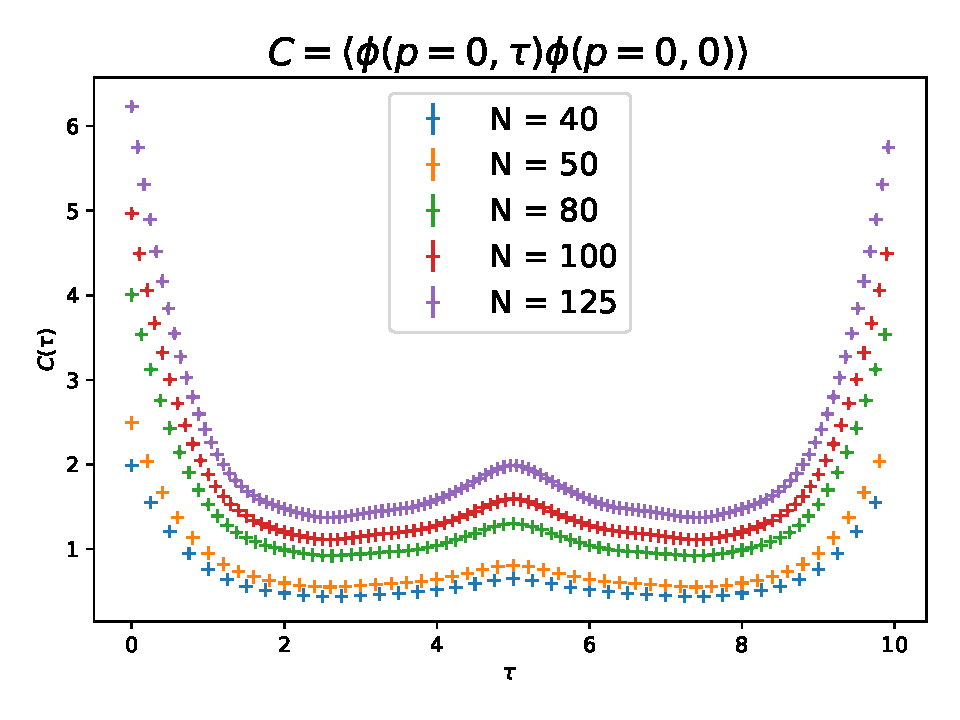
\includegraphics[width=0.5\textwidth]{figures/mass_correlator_plot.pdf}}
        \subfloat[$C(\tau)/C(0)$]{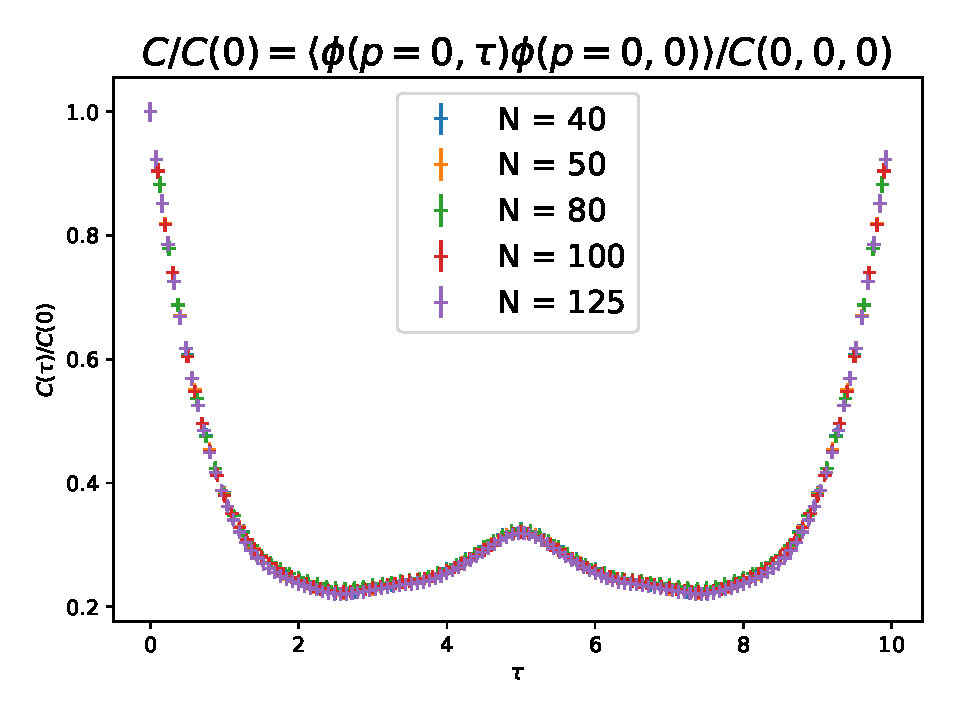
\includegraphics[width=0.5\textwidth]{figures/renorm_mass_correlator_plot.pdf}}
        \caption{Grafico del correlatore $C(\tau, 0, 0)$.}
        \label{fig:mass_correlator_plot}
    \end{figure}

   
    \begin{figure}[htb]
        \centering
        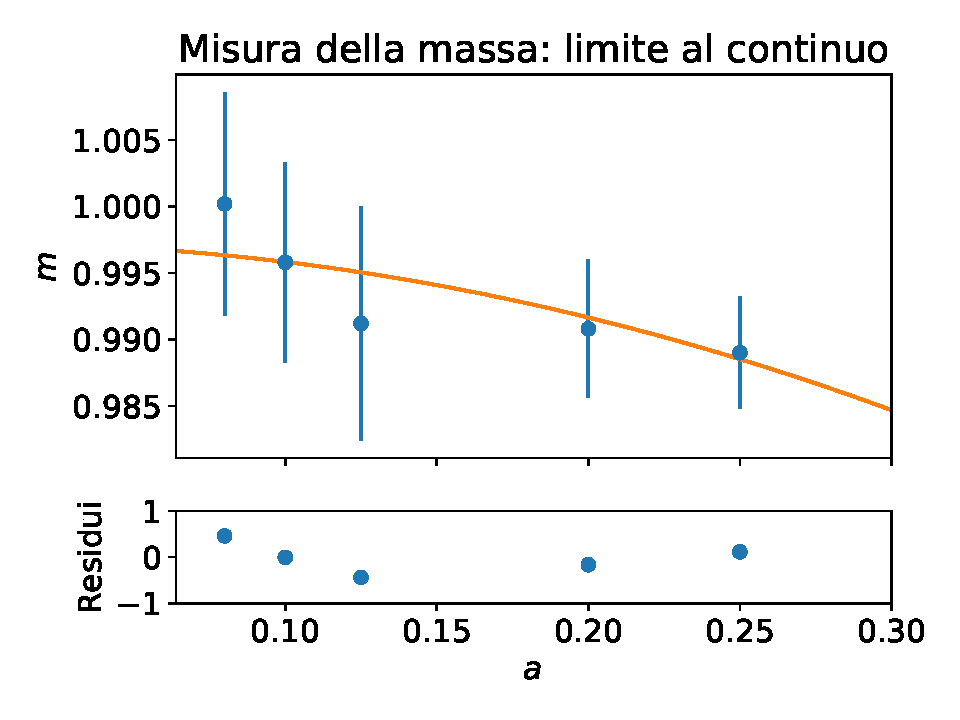
\includegraphics[width=0.7\textwidth]{figures/mass_continuum.pdf}
        \caption{Limite al continuo della misura della massa.}
        \label{fig:mass_fit}
    \end{figure}
    
    Per ogni simulazione, è stato eseguito un fit numerico del correlatore alla funzione $C(\tau) = A \exp (-m_N\tau)$. L'errore su $m_N$ è stato stimato con un algoritmo Bootstrap. Infine, è stato eseguito un fit numerico alla funzione $m(\hat{m}) = m + k \hat{m}^2$ per estrarre il limite del continuo.
    
    Il risultato, riportato in tabella (\ref{tab:mass_fit}) e in figura (\ref{fig:mass_fit}), è in ottimo accordo con quanto previsto, con un $\chindof \simeq 0.15$, che è un po' basso, ed indica una possibile sovrastima degli errori.
    

    

    


\end{document}
